\section{Situazione inziale}

I lavori precedentemente svolti, che hanno contribuito alla definizione di questo percorso, utilizzano due approcci nettamente separati per l'integrazione MAS e GE:
\begin{enumerate}
	\item Implementazione delle caratteristiche dei MAS all'interno della GE, che funge dunque da "contenitore" del MAS stesso;
	\item Realizzazione di un middleware, come layer software, per collegare l'ambiente MAS con GE, che restano quindi separate
\end{enumerate}

\subsection{MAS all'interno di GE} \label{MAS_dentro_GE}

Il primo punto è stato realizzato implementando due modelli tipici dei MAS:
\begin{itemize}
	\item Il modello Beliefs, Desires, Intentions (BDI) per la programmazione degli agenti \cite{amslaurea15657};
	\item Un modello di coordinazione degli agenti tramite spazio di tuple e primitive Linda \cite{amslaurea8424}\cite{amslaurea16100};
\end{itemize}

Il cuore pulsante di entrambi i lavori risiede nell'uso intensivo di un interprete Prolog fatto ad hoc per Unity, UnityProlog \cite{unity_prolog}. Questo interprete dispone di molte funzionalità per estendere l'interoperabilità di Prolog con i GameObject.
Dal momento che è stato progettato per essere usato in maniera specifica con Unity, nasce con delle primitive che permettono di accedere e manipolare GameObject e i relativi componenti direttamente da Prolog. UnityProlog introduce tuttavia alcune limitazioni da tenere bene in considerazione \cite{amslaurea15657}, anche se allo stato attuale è l'unica versione di Prolog del quale è stato dimostrato il corretto funzionamento:
\begin{itemize}
	\item Un interprete per Prolog non sarà mai performante quanto lo può essere un compilatore e questo può rappresentare un problema per simulazioni di MAS piu grandi.
	\item Utilizza lo stack C\# come stack di esecuzione, quindi la tail call optimization non è ancora supportata.
	\item Non supporta regole con più di 10 subgoal, quindi a fronte di una regola complessa con tanti goal da controllare, è necessario frammentare la regola in questione in sotto regole con non più di 10 subgoal per ognuna.
\end{itemize}

\subsection{MAS e GE separati} \label{MAS_GE_separati}

Il secondo percorso si differenzia dal primo per la scelta di lasciare separati GE da MAS realizzando un canale di comunicazione tra i due ambienti. \'E stata introdotta una terminologia per contraddistinguere le entità realizzate sul GE (GameObject) e su MAS (agenti), rispettivamente definite "corpi" e "menti" virtuali \cite{amslaurea12270}.

\medskip

Fondamentalmente un corpo deve eseguire azioni e a seguito di determinati eventi deve trasmettere le proprie percezioni alla mente, mentre la mente deve elaborare le percezioni per decidere quali azioni deve far svolgere al proprio corpo. Per rendere possibile questa comunicazione è stato progettato e implementato un sistema middleware definito secondo il seguente schema.

\begin{figure}[H]
\centering
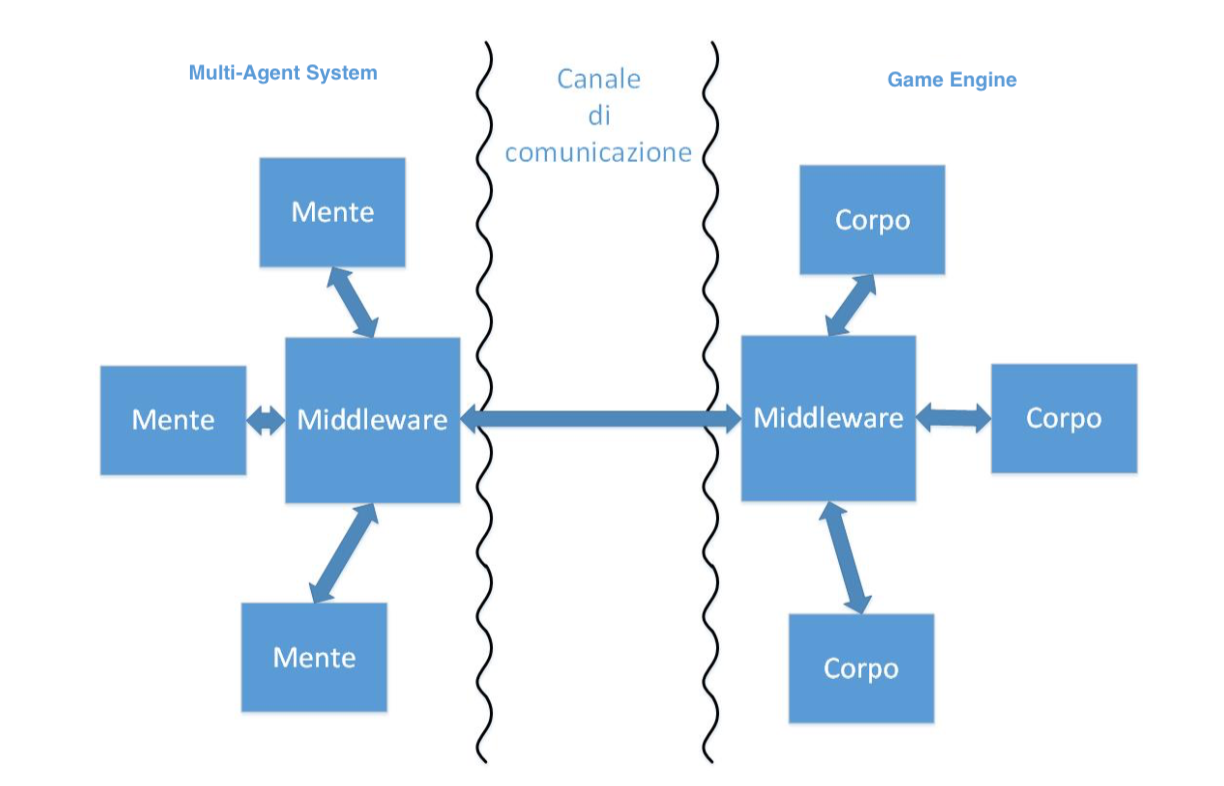
\includegraphics[width=9cm]{figures/Middleware_fuschini.png}
\caption{Il middleware viene suddiviso in due parti, poste sui due lati del canale di comunicazione \cite{amslaurea12270}}
\label{middleware_fuschini}
\end{figure}

Dallo schema (Figura \ref{middleware_fuschini}) si può notare la separazione del middleware nei due sistemi, motivato dalle diverse tecnologie utilizzate dai due ambienti.
 Questa divisione vincola la realizzazione di una nuova parte di middleware in caso di utilizzo di un diversa tipologia di GE e/o MAS.
\medskip

Il protocollo di comunicazione tra le entità è stato realizzato utilizzando messaggi strutturati. Da una parte, le menti devono definire quale azione deve compiere il relativo corpo (es. "muoviti in avanti", "ruota", "prendi", ecc.), dall'altro i corpi devono far sapere alle relative menti le proprie percezioni dell'ambiente circostante (es. "mi ha toccato un entità", "sono alle coordinate 23,12,-6", ecc.) \cite{amslaurea12270}.

\medskip

Nella sezione \ref{architettura_sistema} è definita l'architettura del sistema realizzato evidenziando similitudini e differenze rispetto a questa soluzione. 
